
\begin{problem}[Question:]{Longest Increasing Subarray | Kadan's Algorithm}
    You are given a array of number, find the longest \textbf{subarray} whose sum is maximum.

    \footnotetext{Pratice Link: \href{https://leetcode.com/problems/maximum-subarray/}{LC53}}
    \footnotetext{Solution File: ./resources/subarray-sum.cpp}
\end{problem}

\begin{solution}[Non Recursive DP]
    \rfl{For all subarray problem, please note that iterative solution is the most natural choise.}
    This is same as for all \underline{subsequence} and \underline{subsequence count problem},recursion is the most natural choice.

    \medskip
    \intution{Let $dp[idx,\_]$ be the the maximum subarray sum, that ends at idx \& \textbf{contains idx}.
    Lets try to write up dp[idx] in terms of subproblem.}
    \footnote{i.e assume that we already know the subproblem answer, now just express dp[idx] in terms of subproblems.}
    
    \medskip
    At dp[idx], we have two choices:
    \begin{asparaenum}[(a)]
        \item \indent Continue the previous subarray. $(val_1 = dp[idx-1]+arr[idx])$
        \item Start a new subarray. $(val_2 = arr[idx])$
    \end{asparaenum}

    \begin{marginfigure}
        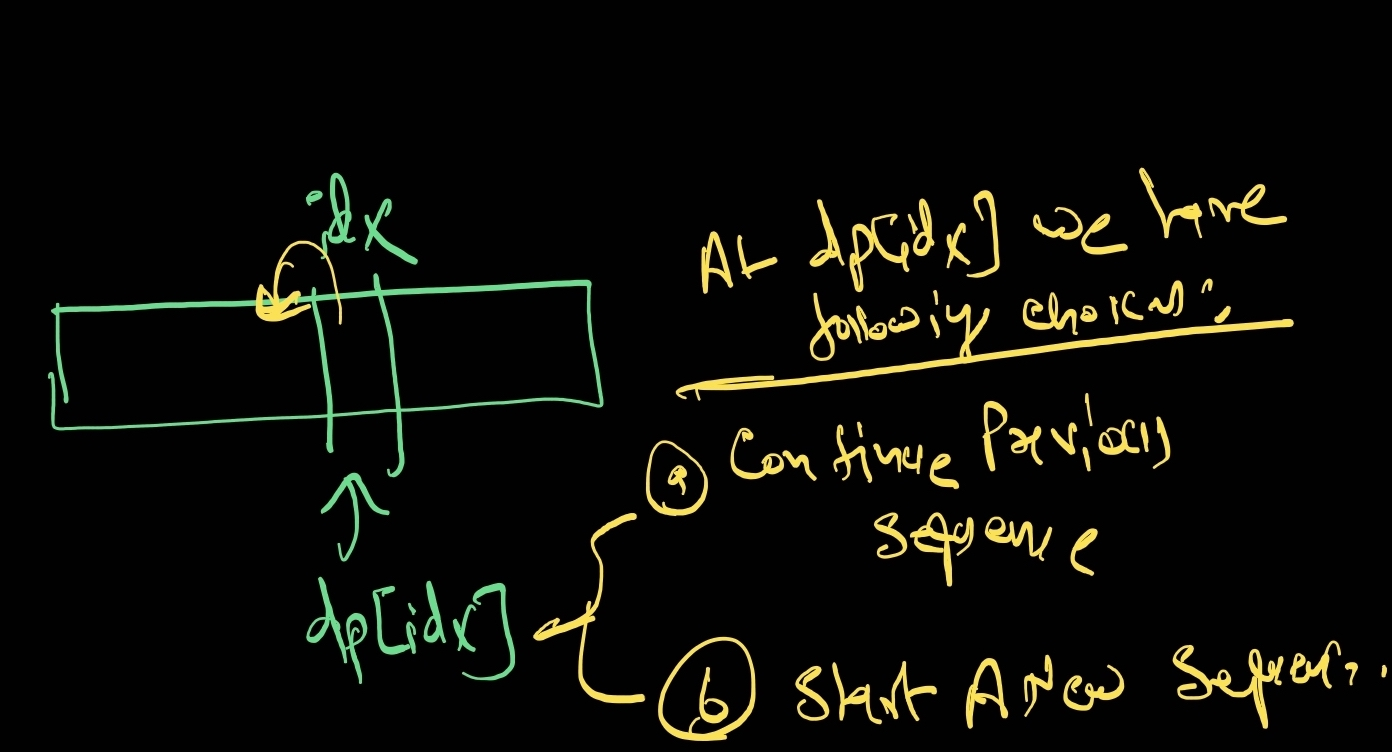
\includegraphics[width=\marginparwidth]{./resources/KadansChoices.jpg}
    \end{marginfigure}

    \medskip
    Hence, for idx we take the best of both $dp[idx] = max(val_1,val_2)$. \\[2mm]
    Now,as we got the maximum subarray when the arr[idx] must be included in the end point of subarray. Our answer be the the maximum amoung all dp[idx].

    \begin{verbatim}
        int maxSubArray(vector<int>& arr) 
        {
            
            int size = arr.size();
            vector<int> dp(arr);
            
            for(int idx=1;idx<size;idx++)
            {
                dp[idx] = max(arr[idx]+dp[idx-1], arr[idx]);
            }

            return *max_element(dp.begin(),dp.end());
    
        }
    \end{verbatim}

\end{solution}

\begin{solution}[Recursive: subarray end at idx]
    Although solving subarray problem in recursive way makes the solution complex.
    Nonetheless, if you want to know how to solve it here is the code.\\[2mm]

    \rfl{
    For subsequence problem, we have recurrance relations as $f(idx)$ := optimal answer for range [0...idx]
    but as this is subarray problem, our $f(idx,_)$ SHOULD be valid only for arr[i...j]}.

    \medskip
    For subarray problem,the defination of recurrance relation changes as \\ \intution{$f(idx,\_)$:= maximum subarray length that ends at idx \& MUST include idx} 
    \medskip

    With above defination of f, at each index idx, we have following options:

    \begin{asparaenum}[(a)]
        \item extends the subarray dp[idx-1] at right \textbf{AND end at idx}.
        \item do not extend the subarray \textbf{and end at idx}.
    \end{asparaenum}

    \begin{code}
        /* we will calculate dp[idx], which is .
        dp[idx] := maximum subarray lenght that ends at idx & MUST include idx*/
        int findAns(int idx,vector<int>& arr)
        {
            if(idx<0) return 0;
            
            if(mem[idx] != INVALID)
                return mem[idx];
            
            int val1 = arr[idx] + findAns(idx-1,arr); //extends the ongoing sub-array & end at idx [start,end] = [...,idx] //extend the subarray at right
            int val2 = arr[idx]; //start the new sub-arrary from this position [start,end] = [idx,ex]
            
          cc  printf("[%d]: (%d,%d)\n",idx,val1,val2);
            
            return mem[idx] = max({val1,val2});
            
        }
    \end{code}
\end{solution}

\begin{solution}[Recursive: subarray start at idx]
    let 
    \intution{$f(idx,\_):=$maximum subarray that starts at idx \& MUST include idx.}

    At each index, we have two option. 
    \begin{asparaenum}[(a)]
        \item Extend the subarray dp[idx+1] at left \textbf{AND start at idx}.
        \item Do not extend the subarray dp[idx+1]. (ie. start a new subarray )
    \end{asparaenum}

    \begin{code}
        /* we will calculate dp[idx], where
        dp[idx]:= maximum subarray that starts at idx & MUST include idx.
        i.e idx is the starting point of the sequence*/
        int findAnsTwo(int idx,vector<int>& arr)
        {
            if(idx >= arr.size()) return 0; //no array => 0 sum
            
            if(mem[idx] != INVALID)
                return mem[idx];
            
            /* both start at arr[idx]*/
            int val1; // use dp[idx+1] to extend the subarray on left side
            int val2; //do not use dp[idx+1] to extend the subarray
            
            val1 = arr[idx] + findAnsTwo(idx+1,arr);
            val2 = arr[idx];
            
            return mem[idx] = max(val1,val2);
        }
    \end{code}
\end{solution}